% latex uft-8
\documentclass[uplatex,a4paper,11pt,oneside,openany]{jsbook}
%
\usepackage[dvipdfmx]{graphicx}
\usepackage[dvipdfmx]{color}
\usepackage{amsmath,amssymb}
\usepackage{enumerate}
\usepackage{bm}
\usepackage{graphicx}
\usepackage{ascmac}
\usepackage{setspace}
\usepackage{here}
\usepackage{multirow}    % セル結合用
\usepackage{tabularx}    % 表用&カラムサイズ指定
\usepackage{comment}
\usepackage{url}
\usepackage{listings,jlisting} %日本語のコメントアウトをする場合jlistingが必要

\usepackage{xcolor}

\definecolor{mygreen}{rgb}{0,0.6,0}
\definecolor{mygray}{rgb}{0.5,0.5,0.5}
\definecolor{mymauve}{rgb}{0.58,0,0.82}

\begin{comment}
\lstset{
  backgroundcolor=\color{white},   % choose the background color; you must add \usepackage{color} or \usepackage{xcolor}; should come as last argument
  basicstyle=\footnotesize,        % the size of the fonts that are used for the code
  breakatwhitespace=false,         % sets if automatic breaks should only happen at whitespace
  breaklines=true,                 % sets automatic line breaking
  captionpos=b,                    % sets the caption-position to bottom
  commentstyle=\color{mygreen},    % comment style
  deletekeywords={...},            % if you want to delete keywords from the given language
  escapeinside={\%*}{*)},          % if you want to add LaTeX within your code
  extendedchars=true,              % lets you use non-ASCII characters; for 8-bits encodings only, does not work with UTF-8
  firstnumber=1000,                % start line enumeration with line 1000
  frame=single,	                   % adds a frame around the code
  keepspaces=true,                 % keeps spaces in text, useful for keeping indentation of code (possibly needs columns=flexible)
  keywordstyle=\color{blue},       % keyword style
  language=Octave,                 % the language of the code
  morekeywords={*,...},            % if you want to add more keywords to the set
  numbers=left,                    % where to put the line-numbers; possible values are (none, left, right)
  numbersep=5pt,                   % how far the line-numbers are from the code
  numberstyle=\tiny\color{mygray}, % the style that is used for the line-numbers
  rulecolor=\color{black},         % if not set, the frame-color may be changed on line-breaks within not-black text (e.g. comments (green here))
  showspaces=false,                % show spaces everywhere adding particular underscores; it overrides 'showstringspaces'
  showstringspaces=false,          % underline spaces within strings only
  showtabs=false,                  % show tabs within strings adding particular underscores
  stepnumber=2,                    % the step between two line-numbers. If it's 1, each line will be numbered
  stringstyle=\color{mymauve},     % string literal style
  tabsize=2,	                   % sets default tabsize to 2 spaces
  title=\lstname                   % show the filename of files included with \lstinputlisting; also try caption instead of title
}
\end{comment}

%ここからソースコードの表示に関する設定
\lstdefinestyle{customc}{
  belowcaptionskip=1\baselineskip,
  breaklines=true,
  numbers=left,
  frame=none,
  xleftmargin=\parindent,
  language=C,
  showstringspaces=false,
  basicstyle=\footnotesize\ttfamily,
  keywordstyle=\bfseries\color{green!40!black},
  commentstyle=\itshape\color{purple!40!black},
  identifierstyle=\color{blue},
  stringstyle=\color{orange},
}

\lstdefinestyle{custompy}{
  belowcaptionskip=1\baselineskip,
  breaklines=true,
  numbers=left,
  frame=single,
  xleftmargin=\parindent,
  language=Python,
  showstringspaces=false,
  basicstyle=\footnotesize\ttfamily,
  keywordstyle=\bfseries\color{green!40!black},
  commentstyle=\itshape\color{purple!40!black},
  identifierstyle=\color{blue},
  stringstyle=\color{orange},
}

\lstdefinestyle{customasm}{
  belowcaptionskip=1\baselineskip,
  frame=L,
  xleftmargin=\parindent,
  language=[x86masm]Assembler,
  basicstyle=\footnotesize\ttfamily,
  commentstyle=\itshape\color{purple!40!black},
}

\lstset{escapechar=@,style=custompy}

\makeatletter
\def\ps@plainfoot{%
  \let\@mkboth\@gobbletwo
  \let\@oddhead\@empty
  \def\@oddfoot{\normalfont\hfil-- \thepage\ --\hfil}%
  \let\@evenhead\@empty
  \let\@evenfoot\@oddfoot}
  \let\ps@plain\ps@plainfoot
\renewcommand{\chapter}{%
  \if@openright\cleardoublepage\else\clearpage\fi
  \global\@topnum\z@
  \secdef\@chapter\@schapter}
\makeatother
%
\newcommand{\maru}[1]{{\ooalign{%
\hfil\hbox{$\bigcirc$}\hfil\crcr%
\hfil\hbox{#1}\hfil}}}
%
\setlength{\textwidth}{\fullwidth}
\setlength{\textheight}{40\baselineskip}
\addtolength{\textheight}{\topskip}
\setlength{\voffset}{-0.55in}
%
\begin{document}
% START DOCUMENT
%
% COVER
\begin{center}
  \huge \par
  \vspace{20mm}
  \huge \par
  \vspace{20mm}
  \LARGE Games with Python \par
  \vspace{100mm}
  \Large \today \par
  \vspace{15mm}
  \Large S.Matoike \par
  \vspace{10mm}
  \Large \par
  \vspace{20mm}
\end{center}
\thispagestyle{empty}
\clearpage
\addtocounter{page}{-1}
\newpage
\setcounter{tocdepth}{3}
% 
\tableofcontents
%
\chapter{はじめに}
%

\chapter{スカッシュ(Squash)ゲーム}

\section{Pygame}

\subsection{Windowの表示}

Window の surface サイズは、横幅WIDTH と高さHEIGHT のタプル (WIDTH, HEIGHT) で指定します。
ここでは、このタプルを WSIZE という名前の変数に納めて使っています

Windowのキャプションを文字列で指定します

キーボード・イべントの取得方法を確認しましょう

\lstinputlisting[caption=Windowを用意する,label=pg01]{../src/pg01.py}

\begin{figure}[h]
\vspace*{-7.5cm}
\hspace*{7.5cm}
\includegraphics[width=0.5\hsize]{./figure/pg01.eps}
%\caption[短い説明]{長い説明}
\label{ラベル}
\end{figure}

%\newpage

【演習】
\begin{enumerate}
\item[(1)] surfaceのサイズを変更して実行してみましょう
\item[(2)] pygame.display.set\_mode()の第2引数にFULLSCREENを指定してみましょう
\item[(3)] キャプションを変えてみましょう
\end{enumerate}

\newpage

\subsection{色の指定と画面の更新}

色の定義は、Red、Green、Blueのそれぞれを256段階(0〜255)で指定したタプルです

1秒あたりの画面更新回数を整数値FPS(Frames Per Second)で指定(1$\le$FPS$\le$30程度)します

pygame.display.update()は、引数を指定しない場合、画面全体を更新します

\lstinputlisting[caption=塗りつぶしの色を指定する,label=pg02]{../src/pg02.py}

\begin{figure}[h]
\vspace*{-11cm}
\hspace*{7.5cm}
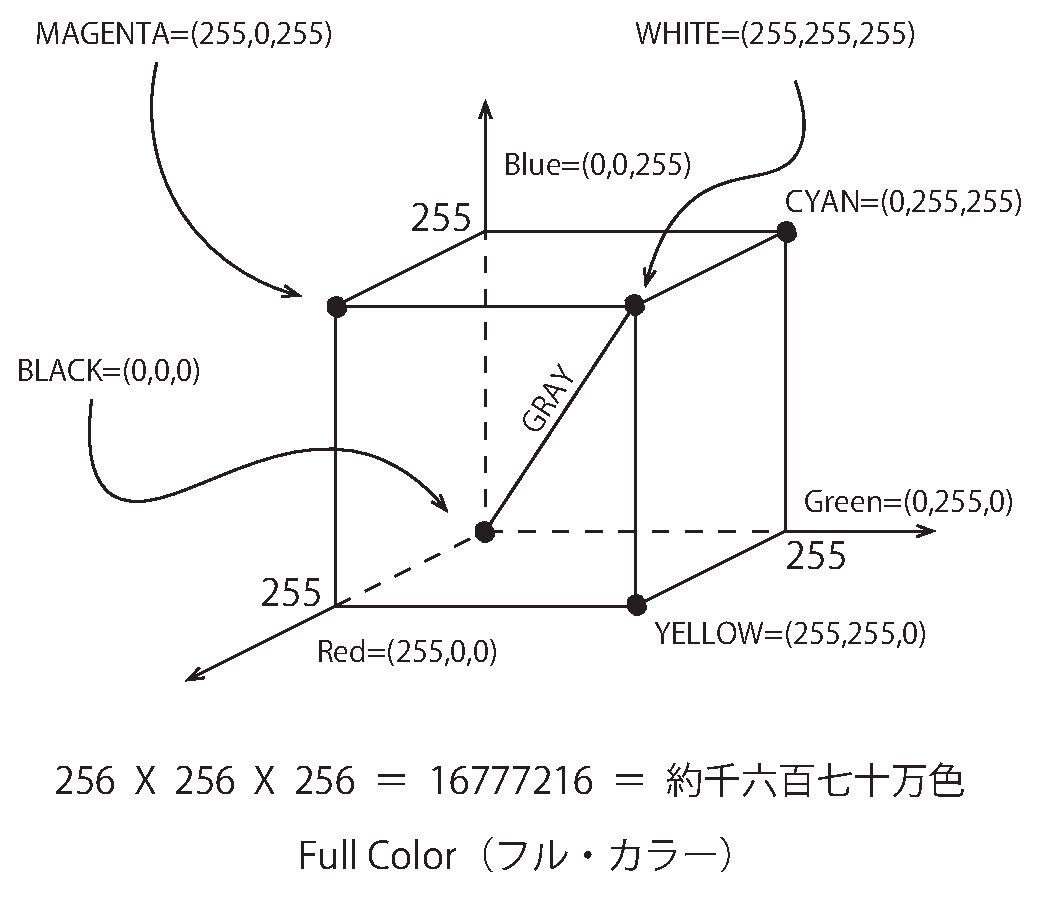
\includegraphics[width=0.5\hsize]{./figure/pg02.eps}
%\caption[短い説明]{長い説明}
\label{ラベル2}
\end{figure}

\vspace{3cm}

n = random.randint(0, 7)は、0$\le$n$\le$7 の範囲の整数をランダムに生成しています

確認のために、print(n) を一行入れてみたら理解の助けになるかもしれません\\

【演習】
\begin{enumerate}
\item[(1)] 白と黒の場合の(Red,Green,Blue)の値を、実際に設定して確認してみよう
\item[(2)] Red,Green,Blueに同じ値を指定すると、灰色の濃さが変わることを確認しよう
\item[(3)] 自分で好みの色を作ってscreenを塗りつぶしてみよう
\item[(4)] FPSの値を変えて実行してみよう
\item[(5)] FPSの値を大きくしすぎると、どんな問題を生じる可能性があるか考えてみよう
\end{enumerate}

\subsection{各種図形の描画}

\begin{center}
\includegraphics[width=0.5\hsize]{./figure/pg04-1.eps}
\end{center}

各種図形を描くときの、共通の引数としてsurfaceとcolorがあります

\begin{itemize}
\item surfaceは、その図形を描画する盤面(pygame.display.set\_modeで生成した)
\item 色の措定colorは、Red,Green,Blueのタプル
\end{itemize}

以下では、個々の図形のそのほかの引数について説明します

\begin{enumerate}

  \item[(1)] 円:pygame.draw.circle(Surface, color, position, radius, width=0)

  \begin{itemize}
  \item 円の中心位置positionは、X座標とY座標のタプル
  \item 円の半径radiusは整数値
  \end{itemize}

  \item[(2)] 線:pygame.draw.line(Surface, color, start\_position, end\_position, width=1)

  \begin{itemize}
  \item 始点start\_positionと終点end\_positionは、各々X座標とY座標のタプル
  \item 線の幅width=1はデフォルト引数(=1なら省略可能)
  \end{itemize}

  \item[(3)] 矩形:pygame.draw.rect(Surface, color, Rect, width=0)

  \begin{itemize}
  \item 線の幅width=0はデフォルト引数(=0なら省略可能)
  \item 矩形を納めるRectは、left, top, width, height のタプル
  \end{itemize}

  \item[(4)] 楕円:pygame.draw.ellipse(Surface, color, Rect, width=0)

  \begin{itemize}
  \item 楕円が収まるRectを、left, top, width, height のタプルで指定
  \end{itemize}

\end{enumerate}

\begin{center}
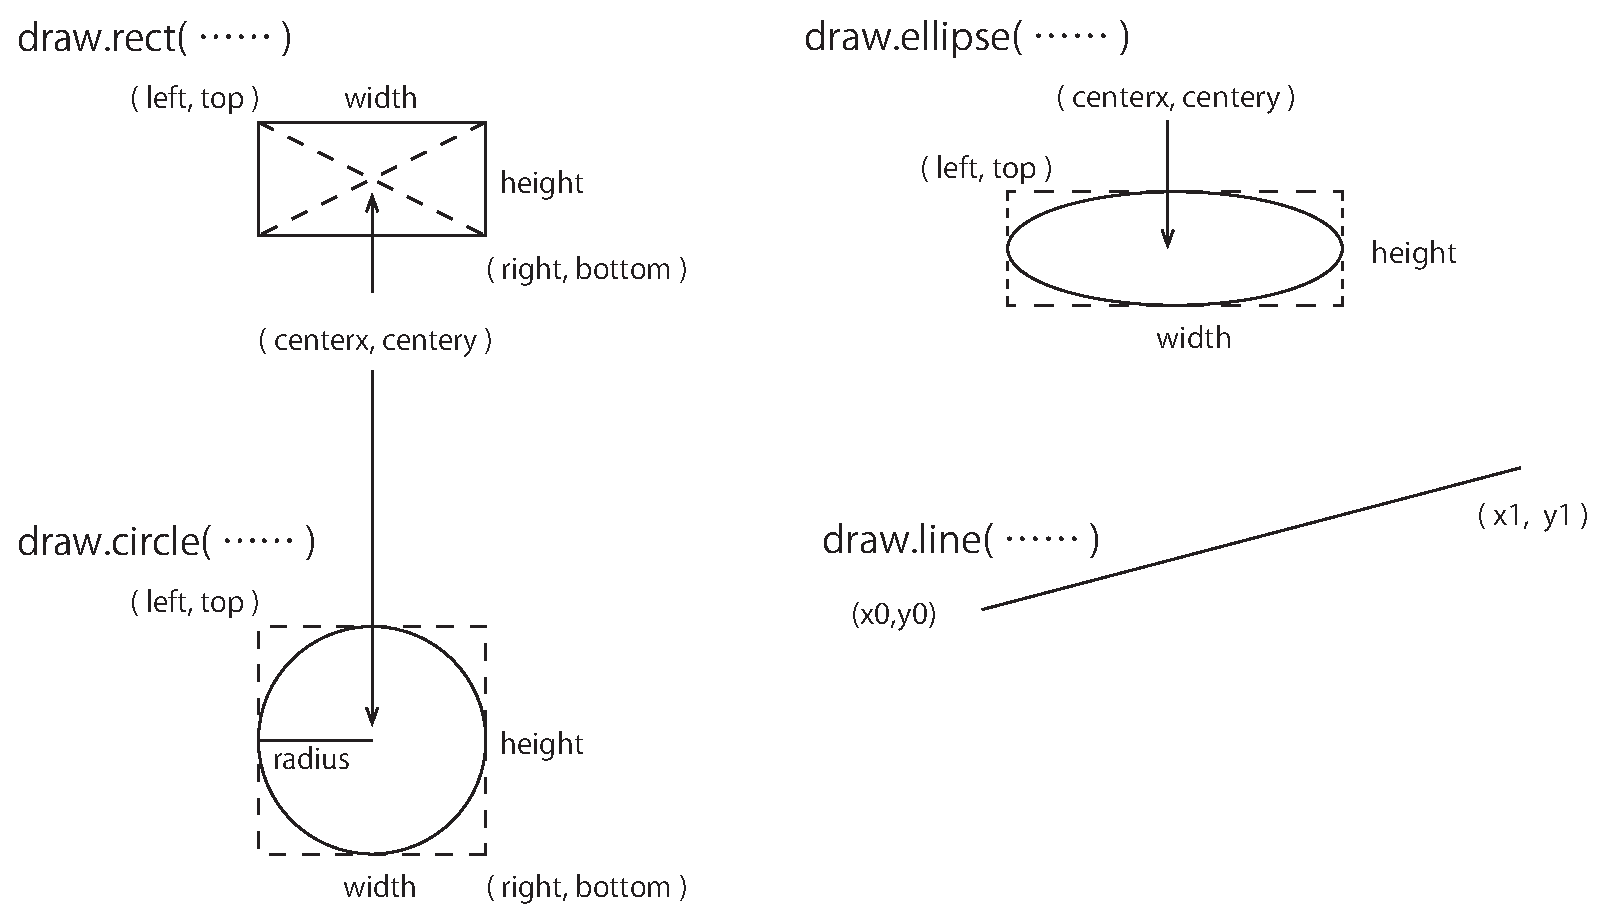
\includegraphics[width=0.6\hsize]{./figure/pg03.eps}
\end{center}

%\newpage

次の作図を試してみましょう
\begin{itemize}
\item surfaceの中央( WIDTH//2, HEIGHT//2)に、半径radius(=100ピクセル)の円Circle
\item surfaceの左上( left=0, top=0 )を始点、右下( right=WIDTH-1, bottom=HEIGHT-1 )を終点とする線Line
\end{itemize}

\begin{lstlisting}[caption=CircleとLine,label=]
import sys
import pygame
from pygame.locals import QUIT

pygame.init()
WIDTH = 640
HEIGHT = 480
WSIZE = (WIDTH, HEIGHT)
surface = pygame.display.set_mode( WSIZE )
pygame.display.set_caption( 'CircleとLine' )
clock = pygame.time.Clock()
FPS = 1

WHITE = (255,255,255)
r = 220
g = 120
b = 0
xc = WIDTH//2
yc = HEIGHT//2
radius = 100
left = top = 0
right = WIDTH - 1
bottom = HEIGHT -1

while True:
    for event in pygame.event.get():
        if event.type == QUIT:
            pygame.quit()
            sys.exit()
    surface.fill( WHITE )
    pygame.draw.circle( surface, (r, g, b), (xc, yc), radius, width=5 )
    pygame.draw.line( surface, (0, 0, 255), (left, top), (right, bottom) )
    pygame.display.update()
    clock.tick( FPS )
\end{lstlisting}

\begin{table}[H]
\vspace*{-0.5cm}
\begin{center}
    \begin{tabular}{cc}
    \includegraphics[width=0.41\hsize]{./figure/linecircle.eps} & \includegraphics[width=0.41\hsize]{./figure/ellipserect.eps}
  \end{tabular}
\end{center}
\end{table}

%\newpage

次の作図を試してみましょう
\begin{itemize}
\item surfaceの中央( WIDTH//2, HEIGHT//2)を四角形Rectの左上の点(left, top)とし、幅widthを100、高さheightを150のRect
\item 上記のRectに収まる楕円Ellipse
\end{itemize}

\begin{lstlisting}[caption=RectとEllipse,label=]
import sys
import pygame
from pygame.locals import QUIT, Rect

pygame.init()
WIDTH = 640
HEIGHT = 480
WSIZE = (WIDTH, HEIGHT)
surface = pygame.display.set_mode( WSIZE )
pygame.display.set_caption( 'RectとEllipse' )
clock = pygame.time.Clock()
FPS = 1

WHITE = (255,255,255)
r = 220
g = 120
b = 0
xc = WIDTH//2
yc = HEIGHT//2
width = 100
height = 150
rect = Rect(xc, yc, width, height)

while True:
    for event in pygame.event.get():
        if event.type == QUIT:
            pygame.quit()
            sys.exit()
    surface.fill( WHITE )
    pygame.draw.line( surface, (0, 0, 255), (0, 0), (639, 479) )
    pygame.draw.line( surface, (0, 0, 255), (639, 0), (0, 479) )
    pygame.draw.rect( surface, (r, g, b), (xc, yc, width, height) )
    pygame.draw.ellipse( surface, (0, 255, 100), rect )
    pygame.display.update()
    clock.tick( FPS )
\end{lstlisting}

【演習】randomをimportして、次のことを試してみましょう
( from random import randint )
\begin{enumerate}
\item[(1)] circleの中心のx座標をrandint(0, WIDTH-1)で、y座標も同様にして作図してみよう
\item[(2)] circleの半径を、乱数randint(1,60)程度で発生させ、中心座標と共に変化させてみよう
\item[(3)] 乱数でr=randint(0,255)、g、bを作り、タプル(r,g,b)でcircleの色を指定してみまよう
\item[(4)] ellipseやrectあるいはlineなどを、乱数を使ってsurface上に表示させてみよう
\item[(5)] surface.fill()をコメントアウトしてみよう
\end{enumerate}%

\begin{center}
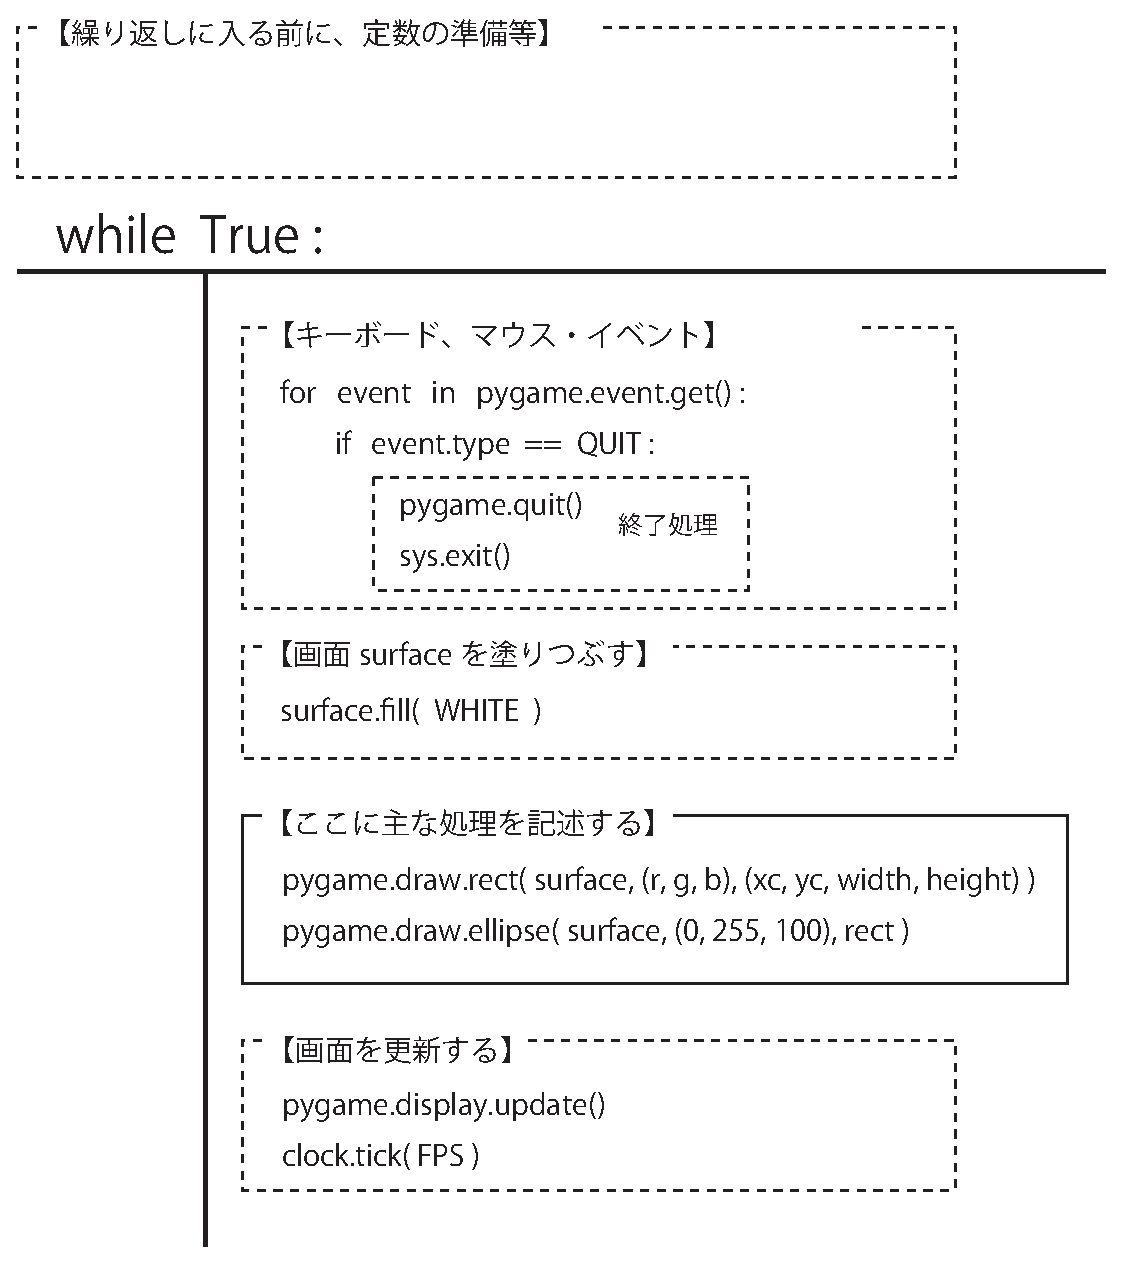
\includegraphics[width=0.6\hsize]{./figure/zushi.eps}
\end{center}

\subsection{図形の移動}

circleで描いたボールの y 座標を、フレーム更新のたびに増加させて、ボールを動かします

ボールの y 座標が、surfaceのHEIGHTに達したら終わります

QUITをイベントとして検出した際に実行される終了処理を、fine()関数にまとめています

surface.get\_rect().width によって得られるのは、WIDTH

surface.get\_rect().height によって得られるのは、HEIGHT

\lstinputlisting[caption=図形の移動,label=pg05]{../src/pg05.py}

\begin{center}
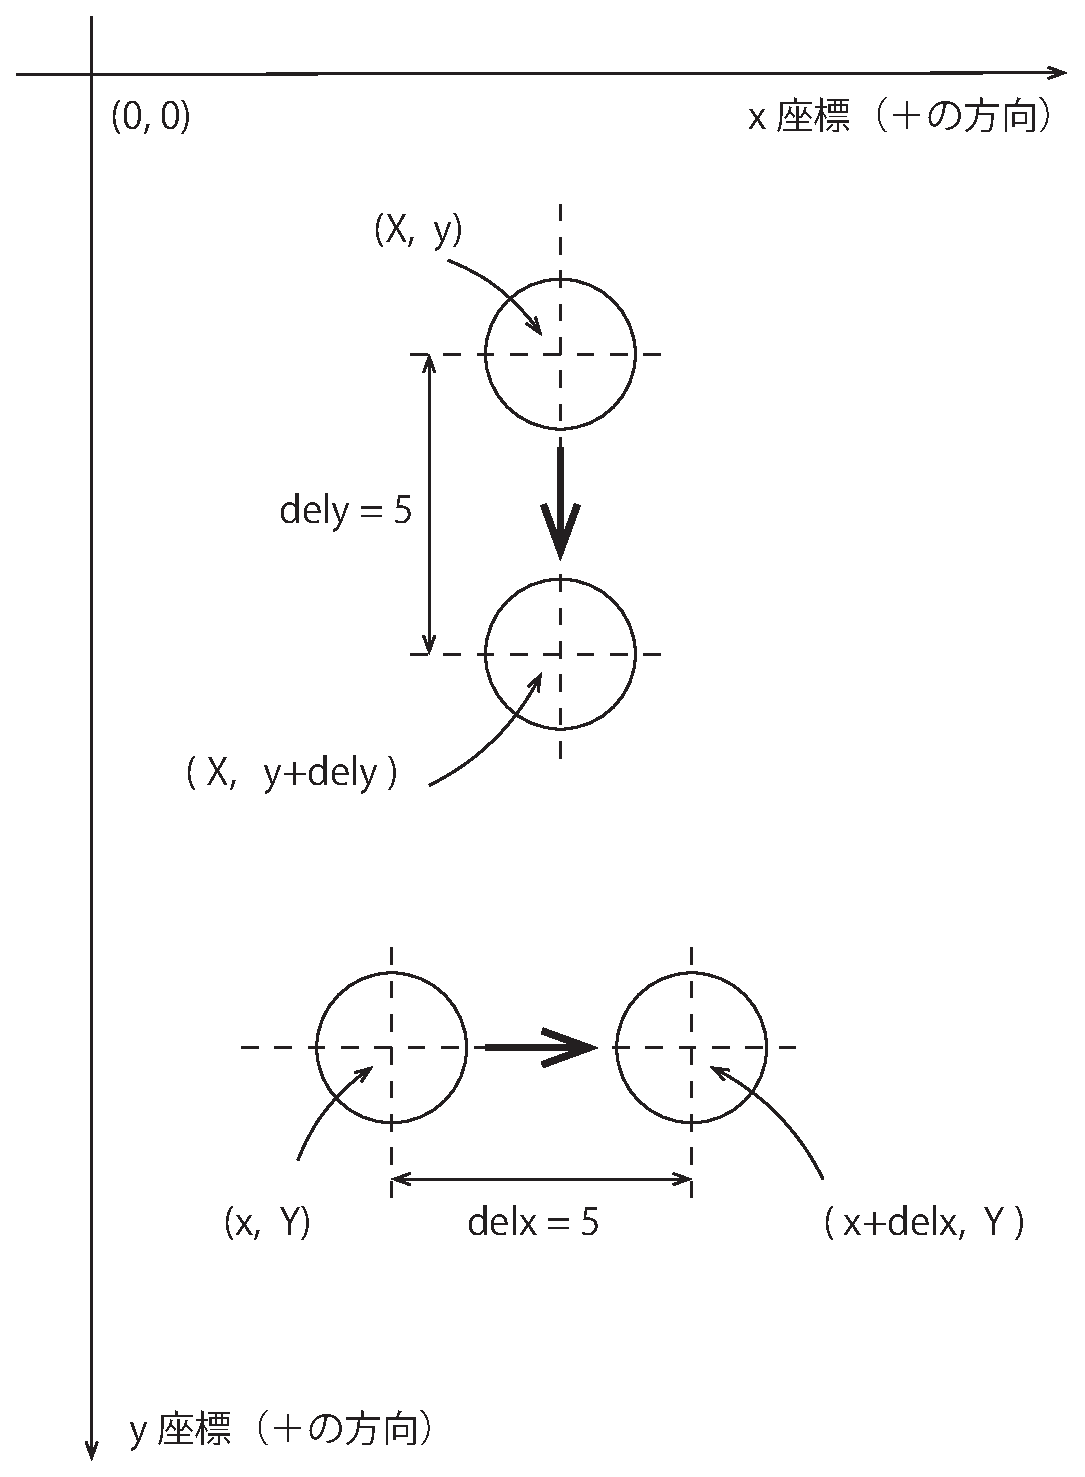
\includegraphics[width=0.4\hsize]{./figure/pg05.eps}
\end{center}

【演習】
\begin{enumerate}
\item[(1)] FPSを変えずにボールの移動するスピードを変えるには、どうすればいいでしょう
\item[(2)] ボールが、画面中央を下から上に動くようにプログラムを書き直してみましょう
\item[(3)] ボールが、画面中央を左から右に動くようにプログラムを書き直してみましょう
\item[(4)] ボールが、画面中央を右から左に動くようにプログラムを書き直してみましょう
\item[(5)] ボールが、画面の左上から右下に向かって動くようにプログラムを書き直してみましょう
\item[(6)] ボールが、画面の左下から右上に向かって動くようにプログラムを書き直してみましょう
\item[(7)] x方向座標値の増分とy方向座標値の増分の値が等しくない様にしたら、ボールの動きはどうなりますか
\end{enumerate}

\subsection{壁で反射するボール}

\begin{center}
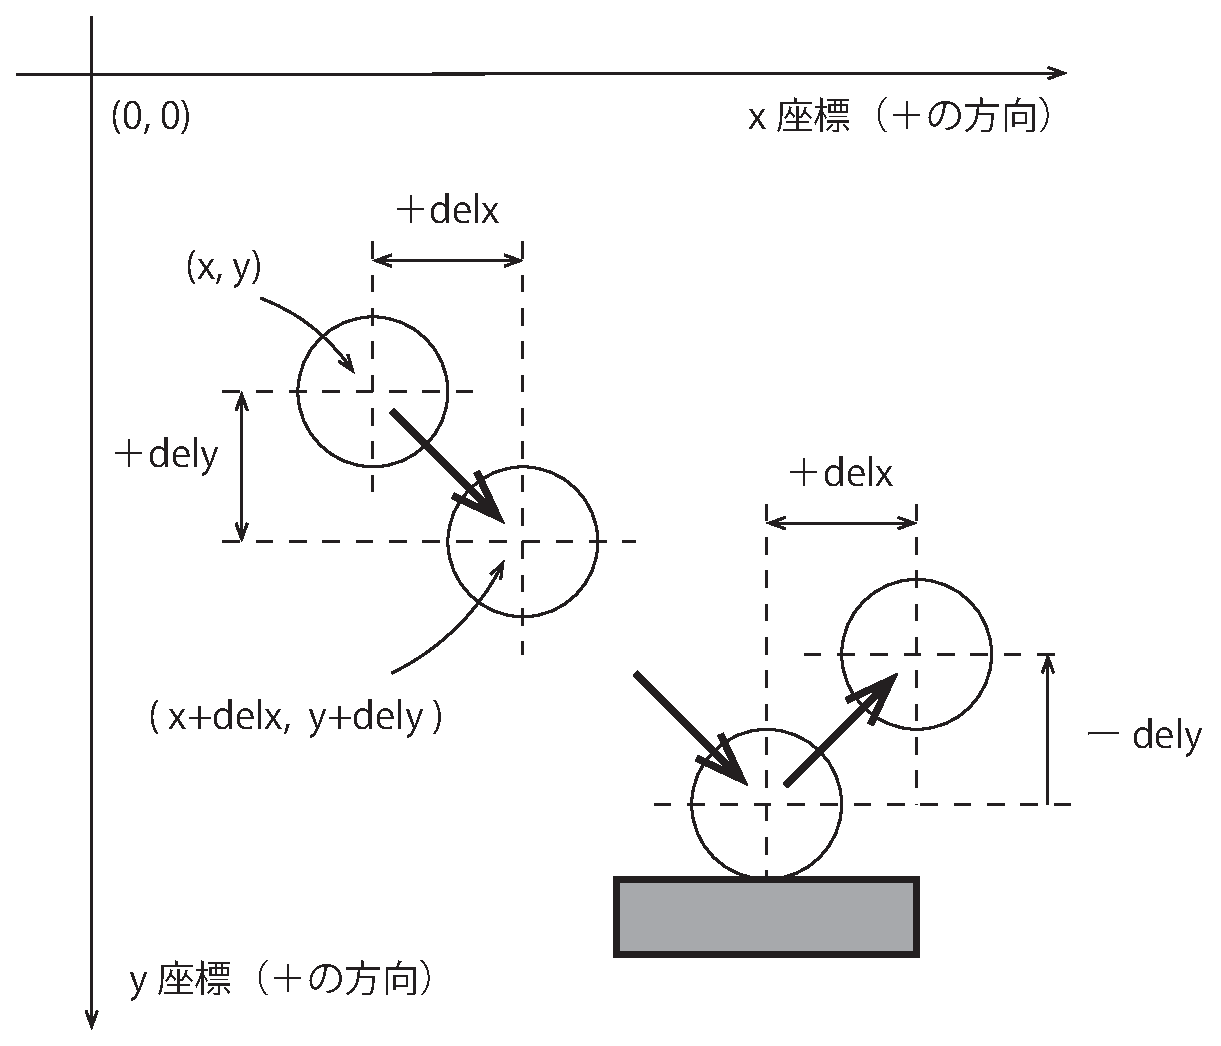
\includegraphics[width=0.5\hsize]{./figure/pg06.eps}
\end{center}

circleで描いたボールの y 座標を、フレーム更新のたびに増加させて、ボールを動かします

ボールの y 座標が、surfaceのHEIGHTに達したら、y 方向の移動量をマイナスの値にしています

ボールの y 座標が、surfaceの上端に達したら、y 方向の移動量をプラスの値に戻しています

\lstinputlisting[caption=反射:位置変化量の符号を反転,label=pg06]{../src/pg06.py}

ボールが上下 y 方向で反射するように、y 方向の移動量の符号を反転しているのは前の例と同じです

ボールを左右 x 方向でも反射するように、x 方向の移動量の符号も反転させています

最初にボールを放出する位置 x 座標を、乱数で決めています

\lstinputlisting[caption=反射,label=pg07]{../src/pg07.py}

\subsection{ラケットの導入}

%\begin{figure}[h]
%\vspace*{-0.85cm}
\begin{center}
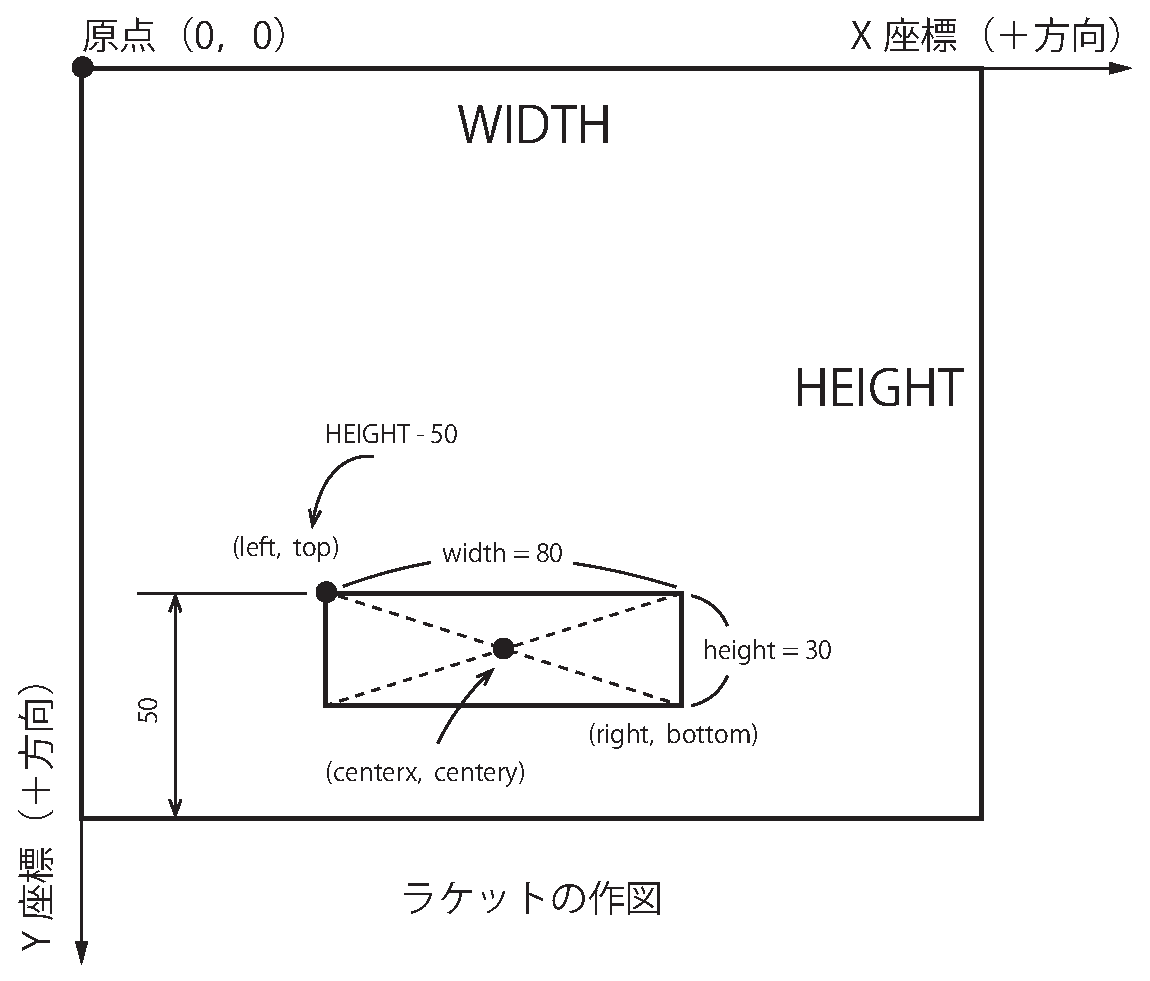
\includegraphics[width=0.5\hsize]{./figure/pg11.eps}
\end{center}
%\end{figure}

ラケットをpygameのRect(クラスのオブジェクト)として作図し、
それを左右の矢印キーを使って動かせるようにします

Rectクラスのオブジェクトは、次の3つの方法のどれかを使って生成できます

\begin{itemize}
\item pygame.Rect( left, top, width, height )
\item pygame.Rect( (left, top), (width, height) )
\item pygame.Rect( Rectオブジェクト )
\end{itemize}

Rectクラスは次のようなプロパティを持っており、値を設定することができます

top, left, bottom, right,
topleft, bottomleft, topright, bottomright,

midtop, midleft, midbottom, midright,
center, centerx, centery, size, width. height, w, h

このプログラム例では、ラケットの初期位置をラケットのRectの左肩(left,top)について、
画面の中央の縦線をleftに、画面の下端から50ピクセル上をtopに、重ねています

また、キーボードからのイヴェントを拾うkey\_event()関数を新たに定義して、
ゲームのメインループの記述を単純にしました

\begin{lstlisting}[caption=ラケットのRectを描画,label=pg08-0]
import sys
import pygame
from pygame.locals import QUIT, Rect
import random

def fine():
    pygame.quit()
    sys.exit()

def key_event():
    for event in pygame.event.get():
        if event.type == QUIT:
            fine()

pygame.init()
WIDTH = 640
HEIGHT = 480
WSIZE = (WIDTH, HEIGHT)
surface = pygame.display.set_mode( WSIZE )
pygame.display.set_caption( 'Squash(Bounding Ball)' )
clock = pygame.time.Clock()
FPS = 20

WHITE = (255,255,255)
# ボールのdraw.circleのために
RED = (255,0,0)
RADIUS = 10
x = random.randint( 0, WIDTH-1 )
y = 0
delx = dely = 5
# ラケットのdraw.rectのために
GREEN = (0,255,0)
SIZE = (WIDTH//2, HEIGHT-50, 80, 10)
racket = Rect( SIZE )

while True:
    key_event()
    surface.fill( WHITE )
    pygame.draw.rect( surface, GREEN, racket )
    pygame.draw.circle( surface, RED, (x,y), RADIUS )
    # 上下の壁でボールの反射
    if y>=HEIGHT or y<0:
        dely = -dely
    # 上下の壁でボールの反射
    if x>=WIDTH or x<0:
        delx = -delx
    # ボールの中心座標を更新
    x += delx
    y += dely
    pygame.display.update()
    clock.tick( FPS )
\end{lstlisting}%

sizeやwidth及びheightの属性の変更は、四角形の大きさを変更することになり、
それ以外のプロパティの変更は、四角形の大きさを変えずに、描画位置を変更することになります

このプログラム例では、ラケットの Rect の centerx プロパティを操作しています

キーボードの左右の矢印キーのイベントを拾って、
右矢印(K\_RIGHT)の時は racket.centerx+=15、左矢印(K\_LEFT)の時は racket.centerx-=15 のように変えることによって、
描画位置を変えています

\lstinputlisting[caption=ラケット,label=pg08]{../src/pg08.py}

\subsection{ラケットとボールの干渉}

ボールの位置はwhile True:のループの中でその都度動いていますから、
毎回ボールのRectを定義し直しては、
ラケットのRect と ボールのRect との間に重なりが生じたか否かを、colliderect()メソッドを使って検出しています

左右方向の矢印キーを押した時、ラケットの動きをスクリーンの幅の中に制限
(ラケットのRectの右側が画面のWIDTH未満であることや、ラケットのRectの左側が画面の左端=0より大きい範囲に制限)
する様にしています

%キーボード・マウスのイベントをチェックしている部分を、関数key\_event()にまとめています
\newpage

\lstinputlisting[caption=ラケットとボールの干渉検出,label=pg09]{../src/pg09.py}

ボールを打ち返し損じた場合、Game Overとprintして終了(whileのループをbreakで抜けてfine()処理に入る)
するようにしています

\subsection{文字テキストの表示}

「Game Over !」の文字テキストを、ゲームっぽく大きな文字で画面の中央に表示させます

textというオブジェクトでは、文字テキストのフォントサイズ、色、表示場所を指定しています

文字の表示位置も、Rectによって幾何情報を保持している点に注目しましょう

font.render()(これはfontオブジェクトのrenderメソッド)は、指定文字を描画したSurfaceを返しますので、
その文字を描画したSurfaceを、下地のSurfaceの上に重ねて描画する必要があります

surface.blit()(これはsurfaceオブジェクトのblitメソッド)は、画像を他の画像の上に重ねて描画するメソッドです

\lstinputlisting[caption=文字テキストの表示など,label=pg10]{../src/pg10.py}

ボールを打ち返し損じた場合、whileのループをbreakで抜けてfine()処理に入ることで
プログラムを終了するようにしているので、せっかくのメッセージを見ることができません
(breakをコメントアウトして、終了の検出はマウスでWindowを閉じるイベントを発生させる
ことに頼るようにしたらよいかもしれません)

ボールを放出する位置のほか、
ボールを放出する方向(左右)も乱数を使って決めています
(具体的には、ボール移動の x 方向の移動量の符号を乱数で決めています)

ラケットでボールをはね返したら10ポイントを加算することとし、
キャプションにその時点での得点を表示するようにしています

\begin{center}
\includegraphics[width=0.4\hsize]{./figure/pg10.eps}
\end{center}

【演習】
\begin{enumerate}
  \item[(1)] 乱数を使って、角度30度〜150度(=180度ー30度)の範囲でボールが放出されるように直してみましょう
  \item[(2)] 青いボールを追加して放出し、2つのボールをラケットで打ち返すゲームに直してみましょう
\end{enumerate}

\newpage

\section{オブジェクト指向}

ここまでに作成してきたプログラムを、オブジェクト指向の考え方を使って書き換えていきます\\

まず、このゲームを構成しているもの(オブジェクト:Object)を列挙して、
それらのもの(オブジェクトあるいはインスタンスとも呼ばれる)が具体的にどのような特性(プロパティー:Property)を持っているのかを考えてみます

とりあえず思いつくものをあげてみると、次の4つでしょうか

\begin{itemize}
  \item ボール:色、形(円)、大きさ(半径)、位置(x,y座標)、スピードなど
  \item ラケット:色、位置(x,y座標)など
  \item 表示するメッセージ:文字列("Game Over!")、色、フォント、サイズ、表示位置(x,y座標)など
  \item スカッシュを行う空間(ボールが飛び交う場):背景色、大きさ(幅、高さ)、キャプションなど
\end{itemize}

基本的に、それぞれのオブジェクトは自分自身の特性(プロパティ)を知って(保持して)いますし、
自分自身のプロパティを操作するメソッド(関数)を持っています。
一方、自分以外のオブジェクトのことは分かりません。つまり他のオブジェクトの情報は持たないようにして、
それぞれのオブジェクトが、できるだけ独立して存在させるようにすると見通しがよくなります。
%(詳しくは「Gofによるデザインパターン」などについて勉強すると良いでしょう)

しかし実際のゲームを考えると、ボールのオブジェクトとラケットのオブジェクトの間の干渉や、
スカッシュ競技場の壁にボールが当たったかどうか、
またボールが後ろ(下)の壁を通り越してしまい、ゲーム終了になったかどうか
など、これらオブジェクトとオブジェクトの間の相互の関わりを調べて操作する必要が生じてきます。

そこで、ゲームの進行を司るものとしてGameというオブジェクトを、
上の4つのオブジェクトに追加して、このゲームを構成することにしましょう

オブジェクトの設計図のことをクラス(Class)といいます

ここから、上で述べた5つのオブジェクトそれぞれについて、クラスの設計を進めていきます

なお、この後クラスから生成される具体的なものを、オブジェクトではなく、インスタンスと呼ぶことがあります

\subsection{main.pyの処理}

if \_\_name\_\_ == '\_\_main\_\_':とかくと、この下の行からプログラムの実行を開始することになります

ここでは、
Gameクラスのオブジェクトであるgameを生成し、その後
gameオブジェクトの中のstart()というメソッドを実行するように指示しています

\begin{lstlisting}[caption=main.py,label=prog01-1]
if __name__ == '__main__':
    game = Game()
    game.start()
\end{lstlisting}%

実際にGameクラスを記述していく際には、
start()メソッドが呼び出されるのですから、Gameクラスの中にstart()メソッドを用意しなければなりません

仮にstart()メソッドでprint()関数だけを実行させることにしますと

\begin{lstlisting}[caption=main.pyとGame.py,label=prog01-2]
class Game:
    def start(self):
        print('Gameクラスのstart()メソッド')

if __name__ == '__main__':
    game = Game()
    game.start()
\end{lstlisting}%

クラスの中に、def \_\_init\_\_(self):として、予め決まった名前のメソッドを定義することができます

このメソッドはコンストラクタと呼ばれ、クラスのオブジェクトが生成される際、最初に一度だけ実行されます

start()メソッドの実行文を\#でコメントアウトしてしまい、gameオブジェクトの生成だけ行ってみると、コンストラクタだけが実行されることが分かります

また、start()メソッドのコメントを外してみると、コンストラクタ実行後にstart()メソッドが実行されることを確認できます

\begin{lstlisting}[caption=main.pyとGame.py,label=prog01-3]
class Game:
    def __init__(self):
        print('Gameクラスのコンストラクタ')

    def start(self):
        print('Gameクラスのstart()メソッド')

if __name__ == '__main__':
    game = Game()
    # game.start()
\end{lstlisting}%

さて、ゲームのプログラム作りに話を戻します

mainプログラムを、まずは次の通り書くことにします

\begin{lstlisting}[caption=main.py,label=p0]
from Game import Game

if __name__ == '__main__':
    game = Game()
    game.start()
\end{lstlisting}

\subsection{画面のクラス:Screen}

Screenクラスでは、スカッシュを行う場所、ボールの飛び交う場を定義します

このクラスが持つ主な特性値(プロパティ)は次の通りです

\begin{itemize}
  \item 画面の幅(WIDTH)
  \item 画面の高さ(HEIGHT)
  \item 描画面(surface)
\end{itemize}

これらの特性値はコンストラクタ(\_\_init\_\_()メソッド)の中で、それぞれの初期値を設定しています

コンストラクタの引数には、デフォルトの値を設定しています

これらの特性値を操作するメソッドは2つです

\begin{itemize}
  \item fillメソッドは、\\fillメソッドによって、引数で受け取ったcolor色でsurfaceを塗りつぶします
  \item captionメソッドは、\\set\_captionメソッドによって、引数で受け取った文字列をWindowのタイトルバーに表示します
\end{itemize}

\begin{lstlisting}[caption=Class Screen,label=p2]
import pygame

class Screen:
    def __init__(self, width=600, height=600):
        self.WIDTH = width
        self.HEIGHT = height
        SIZE = (width, height)
        self.surface = pygame.display.set_mode( SIZE )

    def fill(self, color=(255, 255, 255)):
        self.surface.fill( color )

    def caption(self, str):
        pygame.display.set_caption( str )
\end{lstlisting}

\subsection{ゲームの進行を司るクラス:Game}

ゲームの進行を司るクラスGameは、
今の段階では、そのコンストラクタの中でScreenクラスのオブジェクトをscreenという名前で生成し、それを表示しています

Gameクラスのkey\_event()メソッドでは、Windowを閉じる時のイベントQUITを取得すると、終了処理fine()メソッドを呼び出しています

start()メソッドは、このゲームの主な処理(繰り返し)を行うメソッドなので、この中に具体的なゲームの進行を記述していきます

この後、このGameクラスを少しずつ改造していきます

\begin{lstlisting}[caption=Gameクラス(screenオブジェクトを生成),label=p1]
import sys
import pygame
from pygame.locals import QUIT
from Screen import Screen

class Game():
    WHITE = (255, 255, 255)
    def __init__(self):
        pygame.init()
        self.WIDTH = 640
        self.HEIGHT = 480
        self.screen = Screen( self.WIDTH, self.HEIGHT )
        self.screen.caption( "Squash game" )
        self.clock = pygame.time.Clock()
        self.FPS = 30

    def fine(self):
        pygame.quit()
        sys.exit()

    def key_event(self):
        for event in pygame.event.get():
            if event.type == QUIT:
                self.fine()

    def start(self):
        game_over = False
        while not game_over:
            self.key_event()
            self.screen.fill( Game.WHITE )
            # ↓ ここからゲームの進行を記述していく

            # ↑ ゲーム進行の記述はここまで
            pygame.display.update()
            self.clock.tick(self.FPS)
\end{lstlisting}

クラスの中で定義する関数(メソッドと呼ばれる)の第1引数には、必ず「self」と指定します

selfは、そのクラスから生成される「オブジェクトそれ自身」のことを指しています

「self.変数名」と書いたとき、その変数はオブジェクト変数と呼ばれ、selfすなわち、
クラスから生成された具体的なオブジェクトの中に保持されている変数という意味になります。
そのクラスから複数のオブジェクトが生成された場合には、それぞれのオブジェクトが個別に持っている変数を指していることになります

一方、「self.」を付けていない変数等は、その関数内でだけ通用するローカルな変数になりますので、
当該オブジェクトの中の他のメソッドから参照することはできませんし、またそのクラスの外から参照することもできません

なお、メソッドを呼び出すときは、selfを除いた形で引数を記述します

この他に、「クラス名.変数名」と記述するクラス変数というものがあります。
クラスから生成されるオブジェクトの、いずれにも共通に保持されている変数になります

ここの例では、WHITEというタプルの値をクラス変数として定義し、
fill()メソッドへの引数に Game.WHITE という名前で指定しています

\subsection{ボールのクラス:Ball}

Ballのクラスが持つ特性値(プロパティ)として次のものを考えます

\begin{itemize}
  \item ボールの色(COLOR)
  \item ボールの形(円は楕円ellipseの一種)
  \item ボールの大きさ(円の半径RADIUS)
  \item ボールの現在位置(Rectの特性値、left,top,width,height,およびcenterx,centeryで)
  \item ボールの進む速さ(SPEED)
  \item ボールの進んでいる方向(dirx, diry)
  \item ボールが飛び回る場所(surface)
\end{itemize}

これらのプロパティは、コンストラクタ(\_\_init\_\_()メソッド)の中で、それぞれの初期値を設定しています

コンストラクタの引数には、デフォルトの値を引数として設定していますので、
特別な変更を要しない限り、オブジェクト生成の際にその引数として値を明示的に書く必要がありません

また、Ballクラスは、Rectクラスを継承しているので、
Rectクラスが持っているプロパティ(left、top、centerxなど)は、
そのままBallクラスにある他のプロパティと同じように扱うことができます\\

これらのプロパティを操作するメソッドとして次の5つを用意しました

\begin{itemize}
  \item drawメソッドは、\\ellipse関数を使って、surface上にRectの特性値が保持している現在位置に、指定の色COLORで、円を描画します
  \item stop\_ballメソッドは、\\ボールのSPEEDをゼロにして、ゲーム終了時に呼び出されることを想定しています
  \item movexメソッドは、\\指定のSPEED分だけ、現在ボールが進んでいる方向dirxに、Rectの特性値、即ち現在位置を移動させます
  \item moveyメソッドは、\\指定のSPEED分だけ、現在ボールが進んでいる方向diryに、Rectの特性値、即ち現在位置を移動させます
  \item movexyメソッドは、\\movex関数とmovey関数を順に呼び出して、Rectの特性値、即ちボールの現在位置を移動させます
\end{itemize}

最初に放出されるボールの進行方向を、コンストラクタの中で角度30度〜150度の間の乱数で作り出しています

movex()メソッドやmovey()メソッドでは、ボールの進行方向の角度を、度の単位で持っていることから、
それをラジアン単位に変換した上で、sin()関数やcos()関数を使ってボールの中心座標を計算しています

\begin{center}
  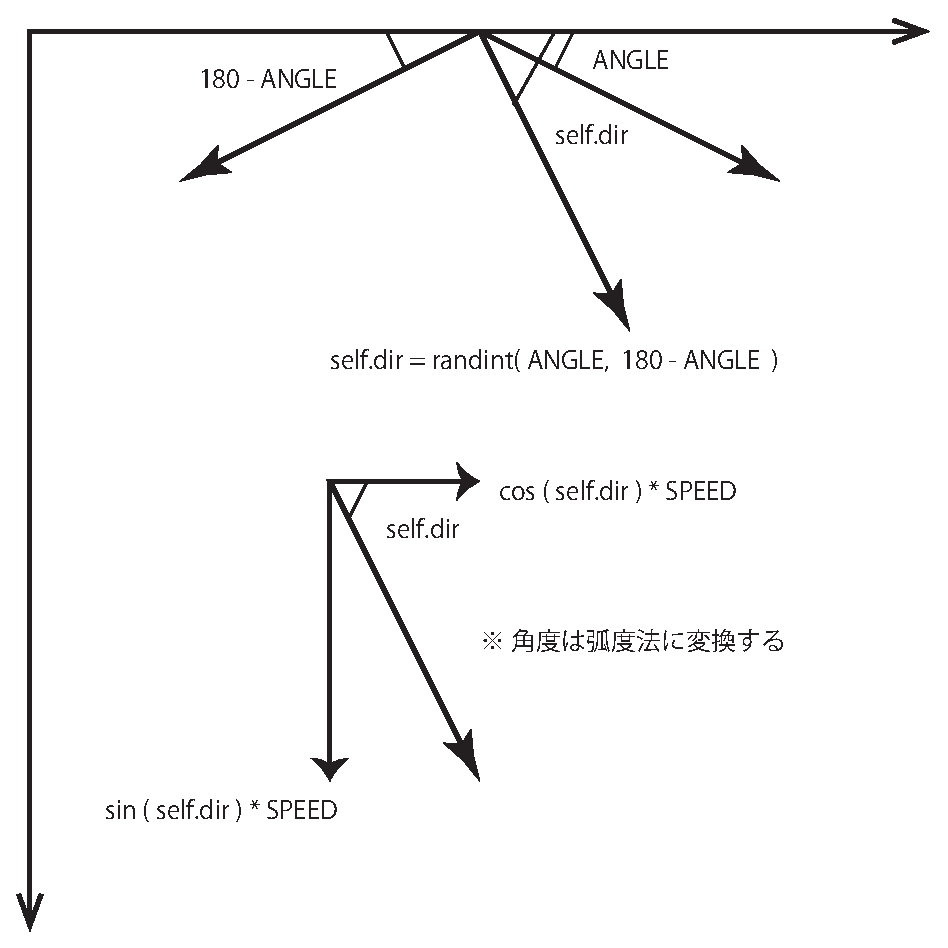
\includegraphics[width=0.4\hsize]{./figure/startball.eps}
\end{center}

\begin{lstlisting}[caption=Ballクラス,label=p3]
from math import sin, cos, radians
from random import randint
import pygame
from pygame.locals import Rect

class Ball( Rect ):
    def __init__(self, surface, color=(180, 180, 180),\
                        diameter=20, speed=10, start=(300,300)):
        self.surface = surface
        self.COLOR = color
        self.SPEED = speed
        ANGLE = 30
        self.dir = randint(ANGLE, 180 - ANGLE)
        self.left = start[0]
        self.top = start[1]
        self.width = diameter
        self.height = diameter

    def stop_ball(self):
        self.SPEED = 0

    def movex(self):
        self.centerx += int( cos(radians(self.dir)) * self.SPEED )

    def movey(self):
        self.centery += int( sin(radians(self.dir)) * self.SPEED )

    def movexy(self):
        self.movex()
        self.movey()

    def draw(self):
        pygame.draw.ellipse(self.surface, self.COLOR, self)
\end{lstlisting}

\begin{center}
  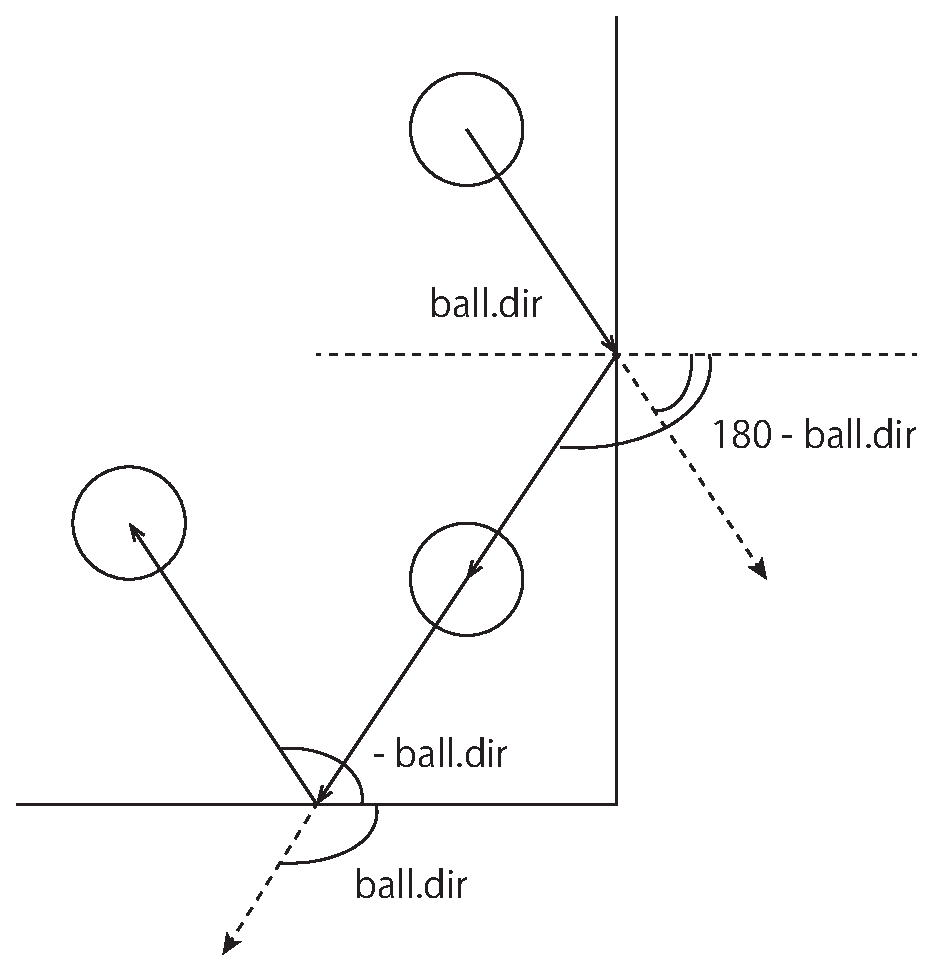
\includegraphics[width=0.4\hsize]{./figure/boundball.eps}
\end{center}

\subsubsection{Gameクラスの書き換え}

Ballクラスのオブジェクト赤いballを、Gameクラスのコンストラクタで生成し、
start()メソッドの中でそのballオブジェクトを描画ball.draw()したり、
ballオブジェクトの現在位置を動かしball.movexy()たりしています

また、Gameクラスのboundary()メソッドでは、
ballオブジェクトがscreenオブジェクトの横幅を超えて移動しようとしたとき、
また、ballオブジェクトがscreenオブジェクトの縦の長さを超えて移動しようとしたときに、
ballオブジェクトの進行方向を反転させています

\begin{lstlisting}[caption=Gameクラス(ballオブジェクトを追加),label=p1]
import sys
import pygame
from pygame.locals import QUIT
from Ball import Ball
from Screen import Screen

class Game():
    WHITE = (255, 255, 255)
    def __init__(self):
        pygame.init()
        self.WIDTH = 640
        self.HEIGHT = 480
        self.screen = Screen( self.WIDTH, self.HEIGHT)
        self.screen.caption("Squash game")
        self.clock = pygame.time.Clock()
        self.FPS = 30
        RED = (255,0,0)
        self.ball = Ball(self.screen.surface, color=RED)

    def fine(self):
        pygame.quit()
        sys.exit()

    def key_event(self):
        for event in pygame.event.get():
            if event.type == QUIT:
                self.fine()

    def boundary(self, ball):
        if not (0 < ball.centerx < self.WIDTH):
            ball.dir = 180 - ball.dir
        if not (0 < ball.centery < self.HEIGHT):
            ball.dir = -ball.dir

    def start(self):
        game_over = False
        while not game_over:
            self.key_event()
            self.screen.fill( Game.WHITE )
            self.ball.draw()
            self.boundary( self.ball )
            self.ball.movexy()
            pygame.display.update()
            self.clock.tick(self.FPS)
\end{lstlisting}

\subsection{ラケットのクラス:Racket}

Racketのクラスに持たせる特性値(プロパティ)は次の通りです

\begin{itemize}
  \item ラケットの色(COLOR)
  \item ラケットの形(長方形Rect)
  \item ラケットの大きさ(Rectの特性値、width,height)
  \item ラケットの現在位置(Rectの特性値、left,top および centerx,centeryで)
  \item ラケットを振り回す場所(surface)
\end{itemize}

これらの特性値はコンストラクタ(\_\_init\_\_()メソッド)で、それぞれの初期値を設定しています

コンストラクタの引数には、デフォルトの値を設定しています

Racketクラスは、Rectクラスを継承しているので、
Rectクラスが持っている特性値(left,topなど)は、
そのままRacketクラスの中にある特性値と同じように扱うことができます\\

これらの特性値を操作するメソッドとして次の3つを用意しました

\begin{itemize}
  \item drawメソッドは、\\rect関数を使って、surface上にRectの特性値が保持している現在位置に、指定の色COLORで長方形を描画します
  \item movexメソッドは、\\引数で受け取ったx方向の移動量delxだけ、Rectの特性値の値、即ち現在位置を移動させます
  \item moveyメソッドは、\\引数で受け取ったy方向の移動量delyだけ、Rectの特性値の値、即ち現在位置を移動させます
\end{itemize}

実は、ラケットはmovey()メソッドを使って動かすことは想定していないので、
movey()メソッドが呼び出されることはありません

\newpage

\begin{lstlisting}[caption=Racketクラス,label=p4]
import pygame
from pygame.locals import Rect

class Racket(Rect):
    def __init__(self, surface, color=(20, 100, 150),\
                       left=300, top=300, width=80, height=10):
        self.surface = surface
        self.COLOR = color
        self.left = left
        self.top = top
        self.width = width
        self.height = height

    def movex(self, delx):
        self.centerx += delx

    def movey(self, dely):
        self.centery += dely

    def draw(self):
        pygame.draw.rect(self.surface, self.COLOR, self)
\end{lstlisting}

\subsubsection{Gameクラスの書き換え}

Gameクラスのコンストラクタで、Racketクラスのオブジェクトracketを生成しています

racketオブジェクトを最初に表示する位置を、leftとtop変数に設定し、Racketクラスのコンストラクタの引数で渡しています

start()メソッドの中で、racketオブジェクトを描画racket.draw()しています

key\_event()メソッドでは、新たに左右の矢印キーが押下されたことを検出するイベント(K\_LEFTとK\_RIGHT)を捉えて、
そこで、racketオブジェクトの表示位置を動かしてracket.movex(移動量)います

その際、racketオブジェクトがscreenオブジェクトの横幅の範囲を超えて移動させることがないように制限しています

BallクラスもRacketクラスも、Rectクラスを継承していたので、
Gameクラスで定義したhitted()メソッドの中では、
ballオブジェクトとracketオブジェクトが干渉したかどうかを、
Rectクラスのcolliderect()メソッドを使って検出することができます

\begin{center}
  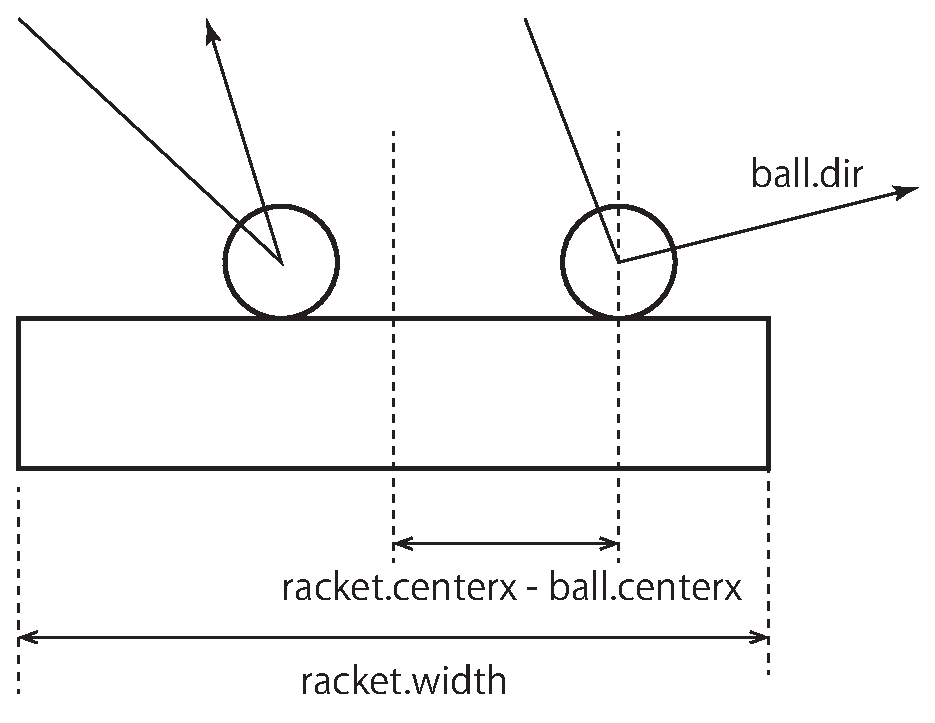
\includegraphics[width=0.4\hsize]{./figure/hitball.eps}
\end{center}
%干渉した場合、ballオブジェクトの進行方向を変えています
\newpage

ボールがラケットに当たった位置が、ラケットの中央から左右どの程度離れているかに応じて、
ボールの反射する方向を変えるようにしています

\begin{lstlisting}[caption=Gameクラス(racketオブジェクトを追加),label=p1]
import sys
import pygame
from pygame.locals import QUIT, KEYDOWN, K_LEFT, K_RIGHT
from Ball import Ball
from Racket import Racket
from Screen import Screen

class Game():
    WHITE = (255, 255, 255)
    def __init__(self):
        pygame.init()
        self.WIDTH = 640
        self.HEIGHT = 480
        self.screen = Screen( self.WIDTH, self.HEIGHT)
        self.screen.caption("Squash game")
        self.clock = pygame.time.Clock()
        self.FPS = 30
        RED = (255,0,0)
        self.ball = Ball(self.screen.surface, color=RED)
        left = self.WIDTH//2
        top = self.HEIGHT - 50
        self.racket = Racket(self.screen.surface, left=left, top=top)
        pygame.key.set_repeat(10, 10)

    def fine(self):
        pygame.quit()
        sys.exit()

    def key_event(self):
        for event in pygame.event.get():
            if event.type == QUIT:
                self.fine()
            elif event.type == KEYDOWN:
                if event.key == K_LEFT and self.racket.left > 0:
                    self.racket.movex(-3)
                elif event.key == K_RIGHT and self.racket.right < self.WIDTH:
                    self.racket.movex(3)

    def hitted(self, racket, ball):
        if racket.colliderect( ball ):
            ball.dir = -(90+(racket.centerx-ball.centerx)/racket.width*100)

    def boundary(self, ball):
        if not (0 < ball.centerx < self.WIDTH):
            ball.dir = 180 - ball.dir
        if not (0 < ball.centery < self.HEIGHT):
            ball.dir = -ball.dir

    def start(self):
        game_over = False
        while not game_over:
            self.key_event()
            self.screen.fill( Game.WHITE )
            self.ball.draw()
            self.racket.draw()
            self.hitted( self.racket, self.ball )
            self.boundary( self.ball )
            self.ball.movexy()
            pygame.display.update()
            self.clock.tick(self.FPS)
\end{lstlisting}

\subsection{メッセージ表示のクラス:Message}

クラスの「継承」を詳しく勉強するために、
メッセージのクラスは、MessageクラスとMessクラスの2段構えにしてみました\\

Messのクラスが持つ特性値(プロパティ)は次の通りです

\begin{itemize}
  \item メッセージの文字列(MESSAGE)
  \item メッセージを表示する場所(XPOS,YPOS)
  \item メッセージの色(COLOR)
  \item メッセージを描画した画面を重ねる下地の画面(surface)
  \item 文字フォント(font)と、そのサイズ(SIZE)
\end{itemize}

文字フォントのサイズは、ここでは固定値(FSIZE=80)にしています

これらの特性値はコンストラクタ(\_\_init\_\_()メソッド)で、それぞれの初期値を設定しています

コンストラクタの引数には、デフォルトの値を設定しています

これらの特性値を操作するメソッドは1つだけです

\begin{itemize}
  \item displayメソッドは、\\Fontのrenderメソッドを使ってMESSAGEを描画し、それを中心座標(XPOS、YPOS)の位置に、COLOR色でsurfaceに重ね合わせます
\end{itemize}

Messクラスを上位のクラスとして継承しているMessageクラスは、
そのコンストラクタで上位のクラスsuper()のコンストラクタを呼び出しています
Messクラスが保持しているMESSAGEプロパティ、XPOS、YPOSプロパティに値を設定しています

また、Gameクラスの中からMessageクラスのdisplay()メソッドを呼び出していますが、
実際は、継承している上位のクラスMessが保持しているdisplay()メソッドが実行されます

\begin{lstlisting}[caption=Messageクラス,label=p4]
import pygame

class Mess:
    def __init__(self, surface, size=80, color=(255,255,0)):
        self.surface = surface
        self.SIZE = size
        self.COLOR = color
        self.font = pygame.font.Font(None, size)
        self.MESSAGE = 'Hello'
        self.XPOS = self.YPOS = 0

    def display(self):
        text = self.font.render(self.MESSAGE, True, self.COLOR)
        textpos = text.get_rect()
        textpos.centerx = self.XPOS
        textpos.centery = self.YPOS
        self.surface.blit(text, textpos)

class Message( Mess ):
    def __init__(self, surface, message, xpos, ypos, size=80, color=(0,0,0)):
        super().__init__(surface, size, color)
        self.MESSAGE = message
        self.XPOS = xpos
        self.YPOS = ypos
\end{lstlisting}

\subsubsection{Gameクラスの書き換え}

Messageクラスのmsg\_goverオブジェクトを、Gameクラスのコンストラクタで生成しています

その際、メッセージ'Game Over!!'の表示色を黄色YELLOWに、表示位置をxposとyposで設定したオブジェクトにしています

コンストラクタでは、メッセージの各情報を設定しただけで、まだ表示していません

実際に表示するのは、boundary()メソッドの中でballオブジェクトがracketオブジェクトに当たらずに、
ballオブジェクトのcenteryプロパティが、screenオブジェクトのHEIGHTプロパティーを超えた時に、
msg\_goverオブジェクトが持っていたMESSAGEプロパティ'Game Over!!'を表示し、
同時に、ballオブジェクトを静止ball.stop\_ball()させています

\begin{lstlisting}[caption=Gameクラス(messageオブジェクトを追加),label=p1]
import sys
import pygame
from pygame.locals import QUIT, KEYDOWN, K_LEFT, K_RIGHT
from random import randint
from Ball import Ball
from Message import Message
from Racket import Racket
from Screen import Screen

class Game():
    WHITE = (255, 255, 255)
    def __init__(self):
        pygame.init()
        self.WIDTH = 640
        self.HEIGHT = 480
        self.screen = Screen( self.WIDTH, self.HEIGHT)
        self.screen.caption("Squash game")
        self.clock = pygame.time.Clock()
        self.FPS = 30
        RED = (255,0,0)
        START = ( randint(0,self.WIDTH-1),0 )
        self.ball = Ball( self.screen.surface, color=RED, start=START )
        left = self.WIDTH//2
        top = self.HEIGHT - 50
        self.racket = Racket(self.screen.surface, left=left, top=top)
        xpos = left
        ypos = self.HEIGHT//2
        YELLOW = (255,255,0)
        self.msg_gover = Message( self.screen.surface, 'Game Over!!',\
                                  xpos, ypos, color=YELLOW )
        pygame.key.set_repeat(10, 10)

    def fine(self):
        pygame.quit()
        sys.exit()

    def key_event(self):
        for event in pygame.event.get():
            if event.type == QUIT:
                self.fine()
            elif event.type == KEYDOWN:
                if event.key == K_LEFT and self.racket.left > 0:
                    self.racket.movex(-3)
                elif event.key == K_RIGHT and self.racket.right < self.WIDTH:
                    self.racket.movex(3)

    def hitted(self, racket, ball):
        if racket.colliderect( ball ):
            ball.dir = -(90+(racket.centerx-ball.centerx)/racket.width*100)

    def boundary(self, ball):
        if not (0 < ball.centerx < self.WIDTH):
            ball.dir = 180 - ball.dir
        if ball.centery < 0:
            ball.dir = -ball.dir
        if self.HEIGHT < ball.centery:
            ball.stop_ball()
            self.msg_gover.display()

    def start(self):
        game_over = False
        while not game_over:
            self.key_event()
            self.screen.fill( Game.WHITE )
            self.ball.draw()
            self.racket.draw()
            self.hitted( self.racket, self.ball )
            self.boundary( self.ball )
            self.ball.movexy()
            pygame.display.update()
            self.clock.tick(self.FPS)
\end{lstlisting}

完成した、OOP版Squashゲームのソースプログラム\\

-rw-r--r--  1 mat  staff   892  2 23 20:30 Ball.py\\
-rw-r--r--  1 mat  staff  2331  2 23 20:33 Game.py\\
-rw-r--r--  1 mat  staff   751  2 23 20:32 Message.py\\
-rw-r--r--  1 mat  staff   540  2 23 20:31 Racket.py\\
-rw-r--r--  1 mat  staff   368  2 23 20:29 Screen.py\\
-rw-r--r--  1 mat  staff    86  2 23 20:29 main.py\\


%\lstinputlisting[caption=Squashゲームの完成,label=squash]{squashobj1.py}
%\section*{謝辞}
%\addcontentsline{toc}{chapter}{謝辞}
%
\begin{thebibliography}{99}
  \bibitem{1} Brett Slatkin 著、黒川利明 訳(オライリー・ジャパン) 「Effective Python 第2版」
  \bibitem{2} 辻真吾、小林秀幸、鈴木庸氏、細川康博 著(技術評論社)Python3 スキルアップ教科書
  \bibitem{3} 金宏和實 著(日経BPマーケティング)「はじめるPython!,ゼロからのゲームプログラミング」
  \bibitem{4} 田中賢一郎 著(インプレスR\&D)「ゲームを作りながら楽しく学べるPythonプログラミング」
\end{thebibliography}
%
% END DOCUMENT
\end{document}
%
